\documentclass{article}
\title{Disaster Event Analysis using X Tweets}
\author{Bryan Alexis Ambriz}
\date{September 2023}
\usepackage[style=authoryear, backend=biber]{biblatex}
\addbibresource{disaster_event_analysis_using_x_tweets.bib}
\usepackage{graphicx}
\addbibresource{disaster_event_analysis_using_x_tweets.bib}
\begin{document}
\maketitle
\section{Introduction to KDD Methodology}
\paragraph{The KDD methodology, short for Knowledge Discovery in Databases, offers a structured approach to analyzing and extracting valuable insights from extensive datasets. It is commonly employed in disaster event analysis among other applications. Knowledge Discovery in Databases (KDD) is a comprehensive process focused on extracting meaningful patterns from vast datasets. When dealing with text data, KDD presents unique challenges and opportunities. Text data, inherently unstructured, differs from numerical or categorical datasets, demanding specialized preprocessing and analysis techniques. Common tasks include tokenization, stemming, and stop word removal, which simplify the text and make it more amenable for pattern recognition. Beyond preprocessing, text data often requires transformation into a structured format, such as a term-document matrix or TF-IDF representation. Techniques like topic modeling, sentiment analysis, and association rules become especially pertinent. Discovering patterns in the text can unveil trends, sentiments, and emerging themes, making it invaluable for various domains ranging from market research to public health.}
\section{Understanding Data Preprocessing in Python}
\paragraph{Data preprocessing is a vital step in the KDD methodology, as it involves transforming raw data into a structured format that can be analyzed effectively. In the context of disaster event analysis using tweets, Python provides a set of powerful tools and libraries to preprocess the text data. For example, in the case of this project, I used Python's Pandas, Zipfile, MatPlotLib, Seaborn, and Wordcloud libraries. These libraries help in tasks such as loading and manipulating the data, extracting relevant information, cleaning and transforming the text data, and visualizing the patterns and insights extracted from the data.}
\section{Exploring Disaster Events through Social Media Data}
\paragraph{Social media platforms, specifically X, have emerged as valuable sources of information during disaster events. Analyzing tweets related to disaster events can provide real-time and on-the-ground insights into the impact, response, and recovery efforts. By applying the KDD methodology to tweets, researchers can uncover patterns and insights that are crucial for understanding the dynamics of disaster events. The process of preprocessing the tweets involves several steps to ensure that the data is clean and ready for analysis.}
\section{Patterns and Insights from Preprocessed Tweets}
\paragraph{After preprocessing the tweets related to disaster events using Python, several patterns and insights can be gleaned from the data. For example, the frequency of certain words or phrases can indicate the severity or type of disaster event. In this project, we feature engineered 5 new features that were not present in the data are taken from the Kaggle ''Natural Language Processing with Disaster Tweets" page. These new features include "tweetlength", "avgwordlength", "hashtagcount", "mentioncount", and "urlcount". Additionally, through the use of exploratory analysis techniques, we identified key location-based topics or themes present in the tweets. For example, we discovered that during hurricane or tornado events, tweets often coincide with particular locations where the disaster is occurring, such as specific cities or regions. These location-based insights can be valuable in emergency response efforts, as they help understand the geographical extent of the disaster and inform resource allocation decisions.}
\section{Visualizing Disaster Events using Python}
\paragraph{To visualize the patterns and insights extracted from preprocessed tweets related to disaster events, we utilized various Python libraries such as Matplotlib, Seaborn and Wordcloud. We plotted various charts and visualizations to present the information clearly and concisely.}
\paragraph{This is a word cloud of the most frequently used words in the preprocessed tweets related to disaster events.}
\begin{figure}[h]
    \centering
    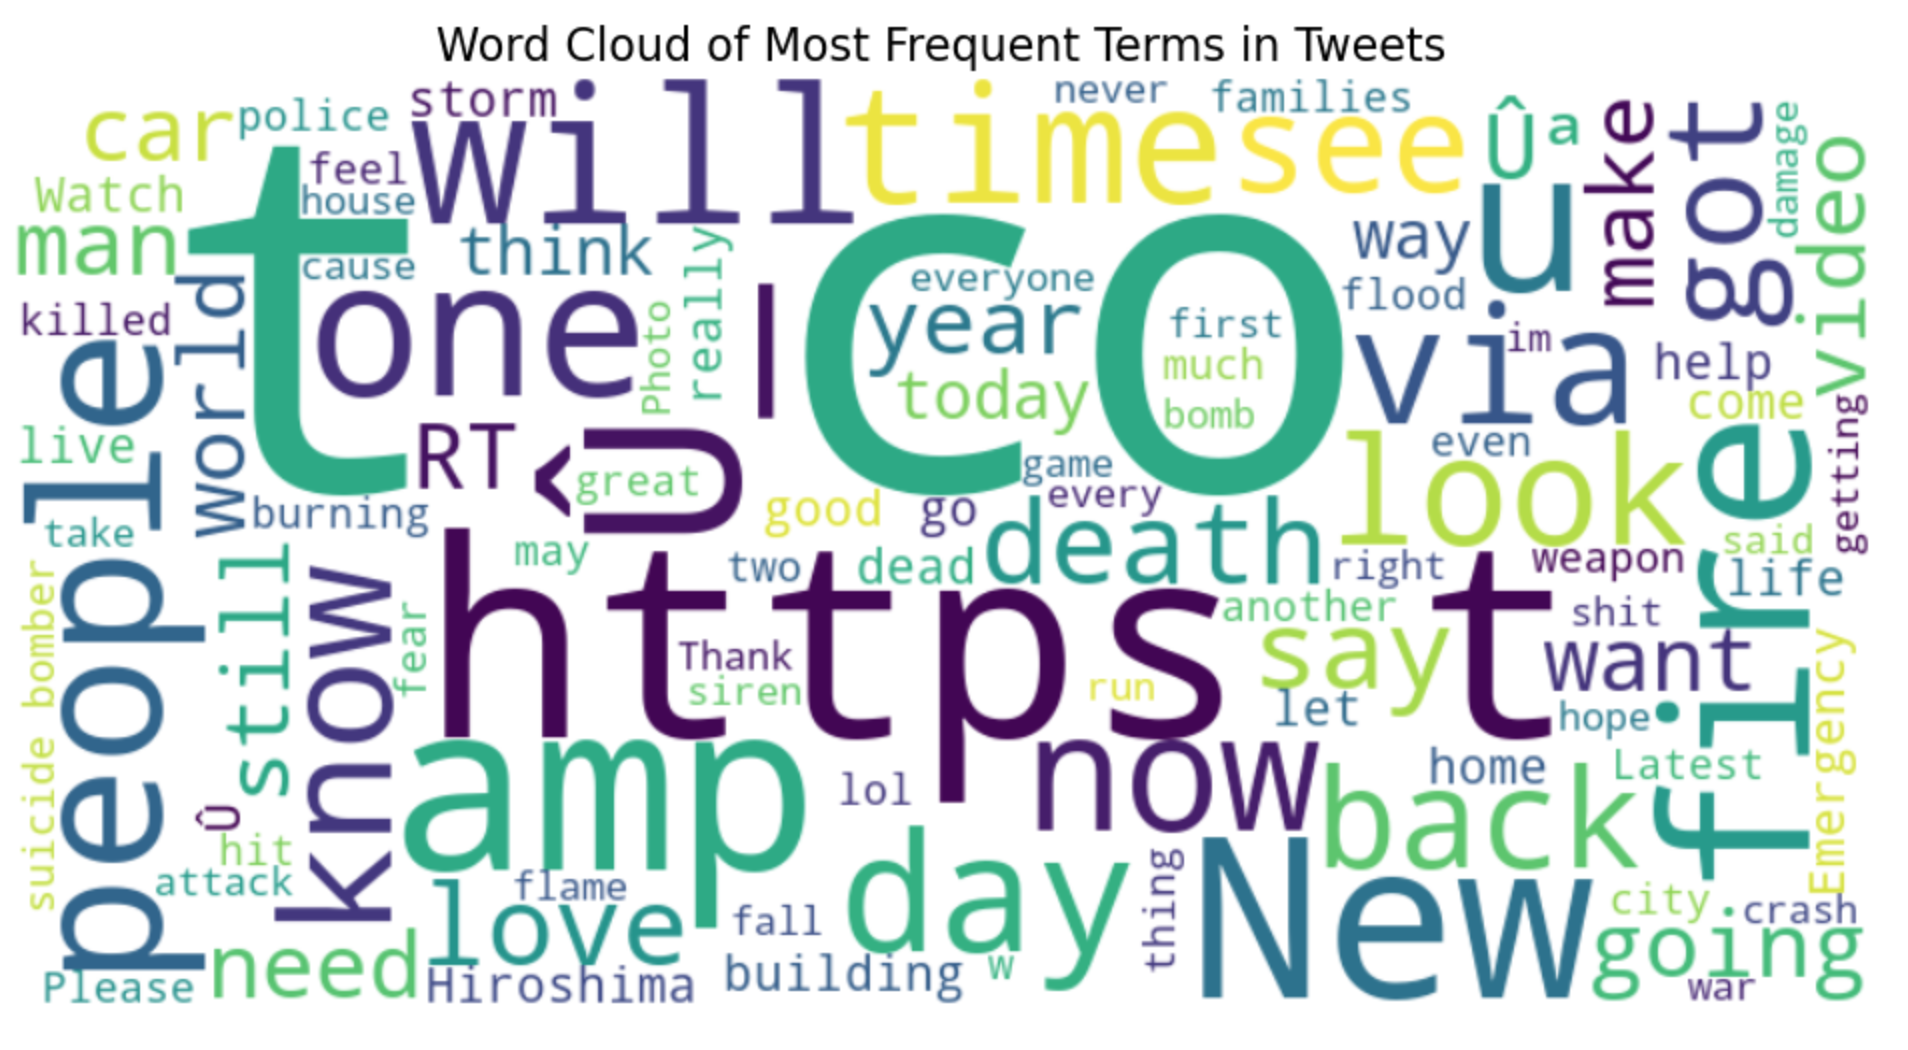
\includegraphics[width=0.8\textwidth]{wordcloud_tweets.png} 
    \caption{Word Cloud of Disaster Keywords}
    \label{fig:my_label}
\end{figure}
\paragraph{This word cloud provides a visual representation of the most commonly used words in the tweets, allowing us to quickly identify the main themes and topics.}
\paragraph{We also used Matplotlib to visualize the top 10 locations with the most diverse disaster tweets, as well as the frequency distribution of the top 20 disaster keywords.}
\begin{figure}[h]
    \centering
    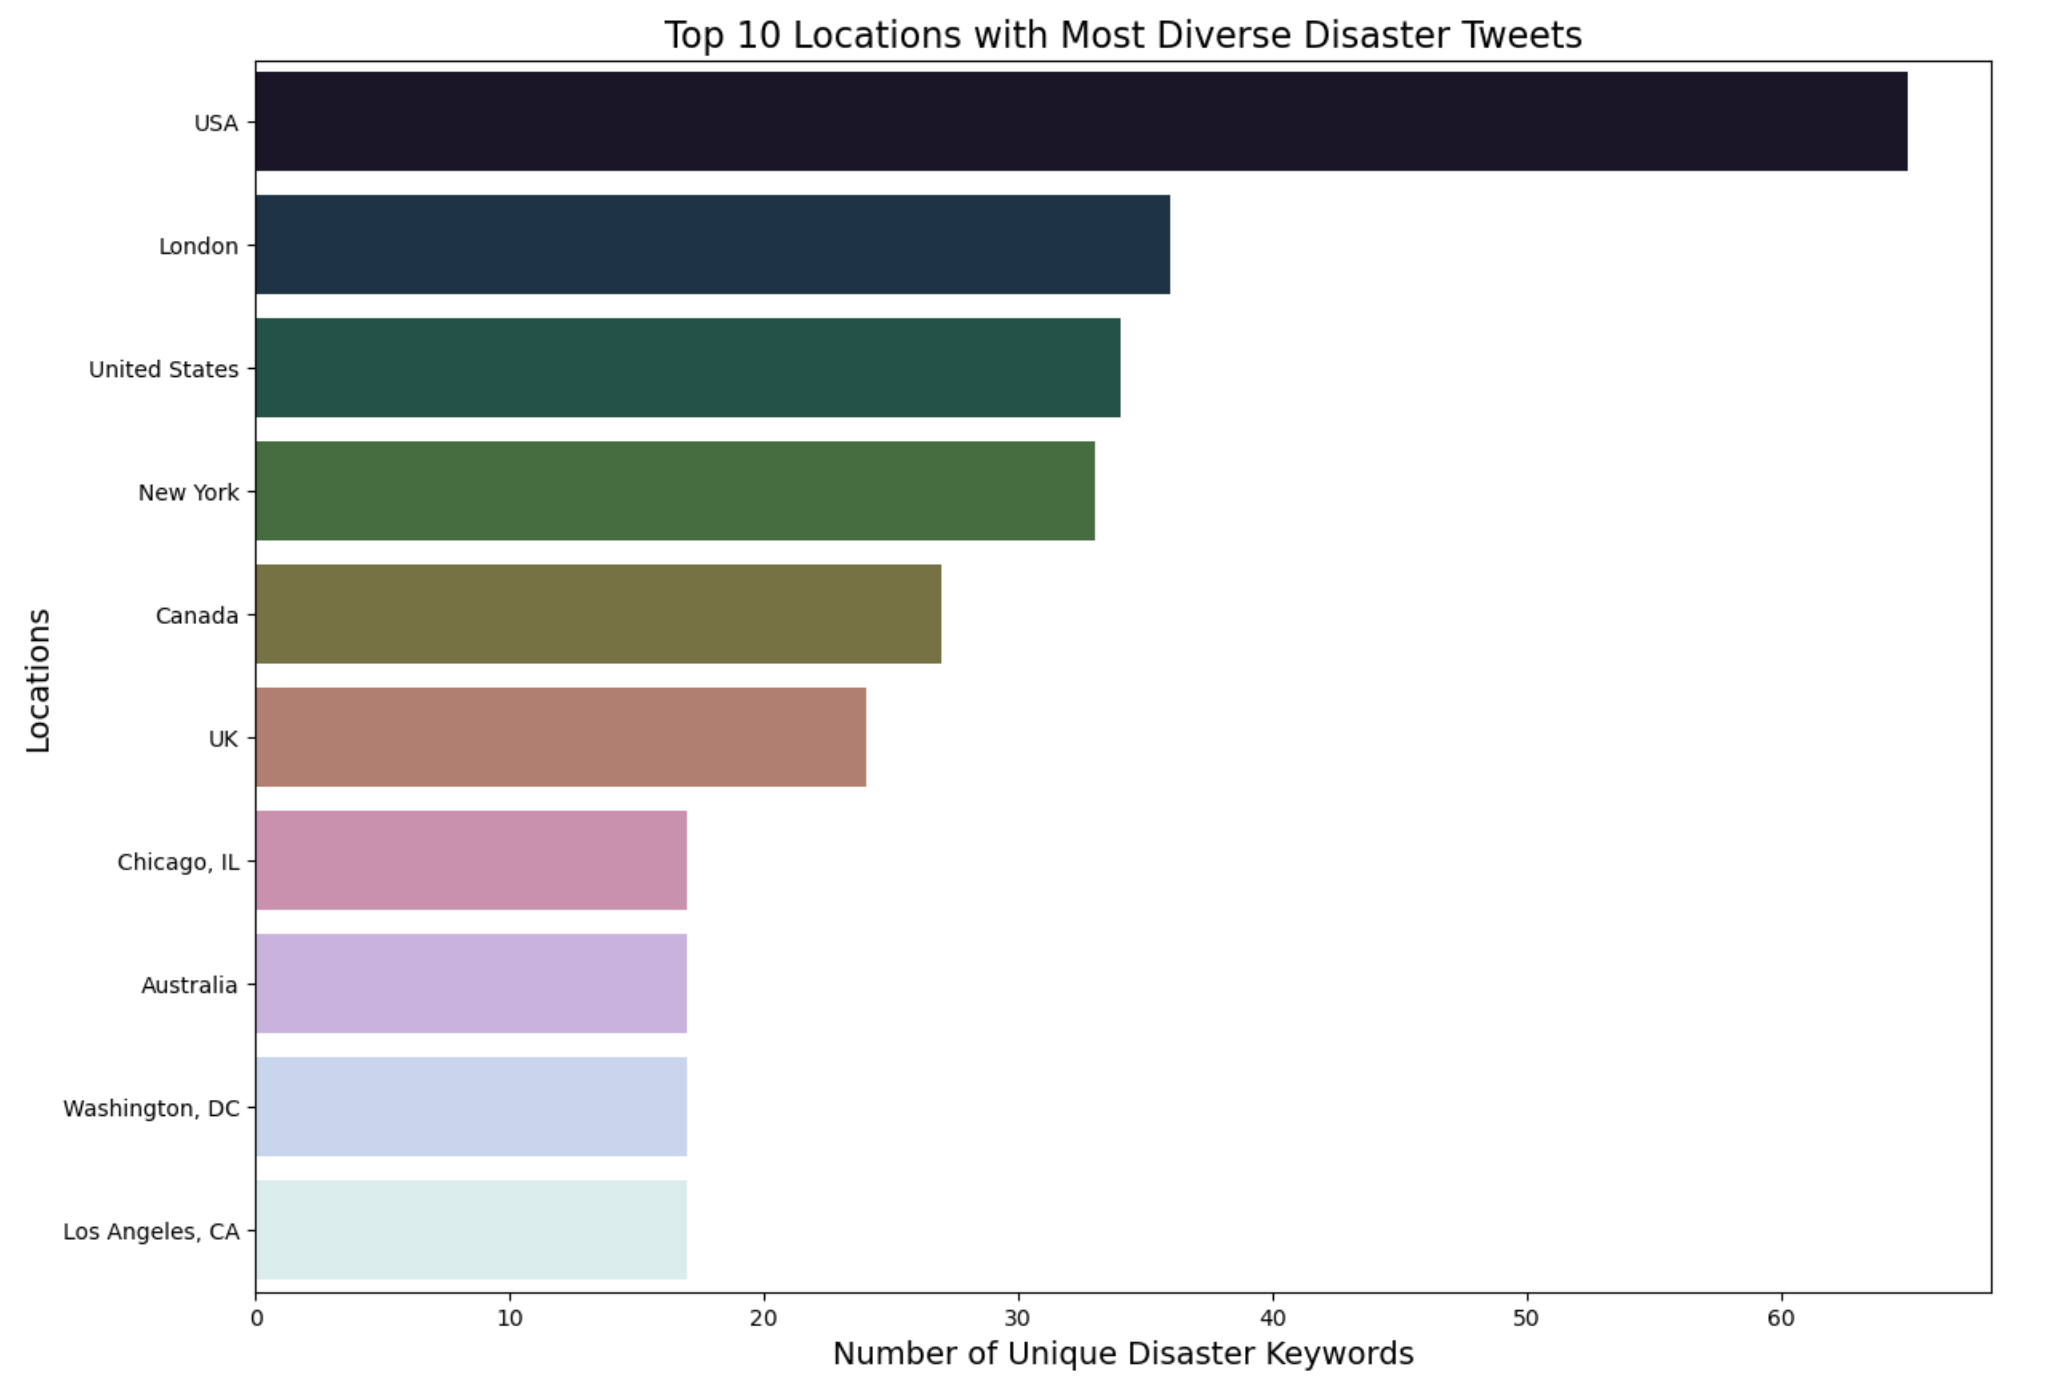
\includegraphics[width=0.8\textwidth]{top_10_locations.png}
    \caption{Top 10 Locations}
    \label{fig:my_label}
\end{figure}
\paragraph{By analyzing the top locations with the most diverse disaster tweets, we can identify the areas that are most affected by various disasters.}
\begin{figure}[h]
    \centering
    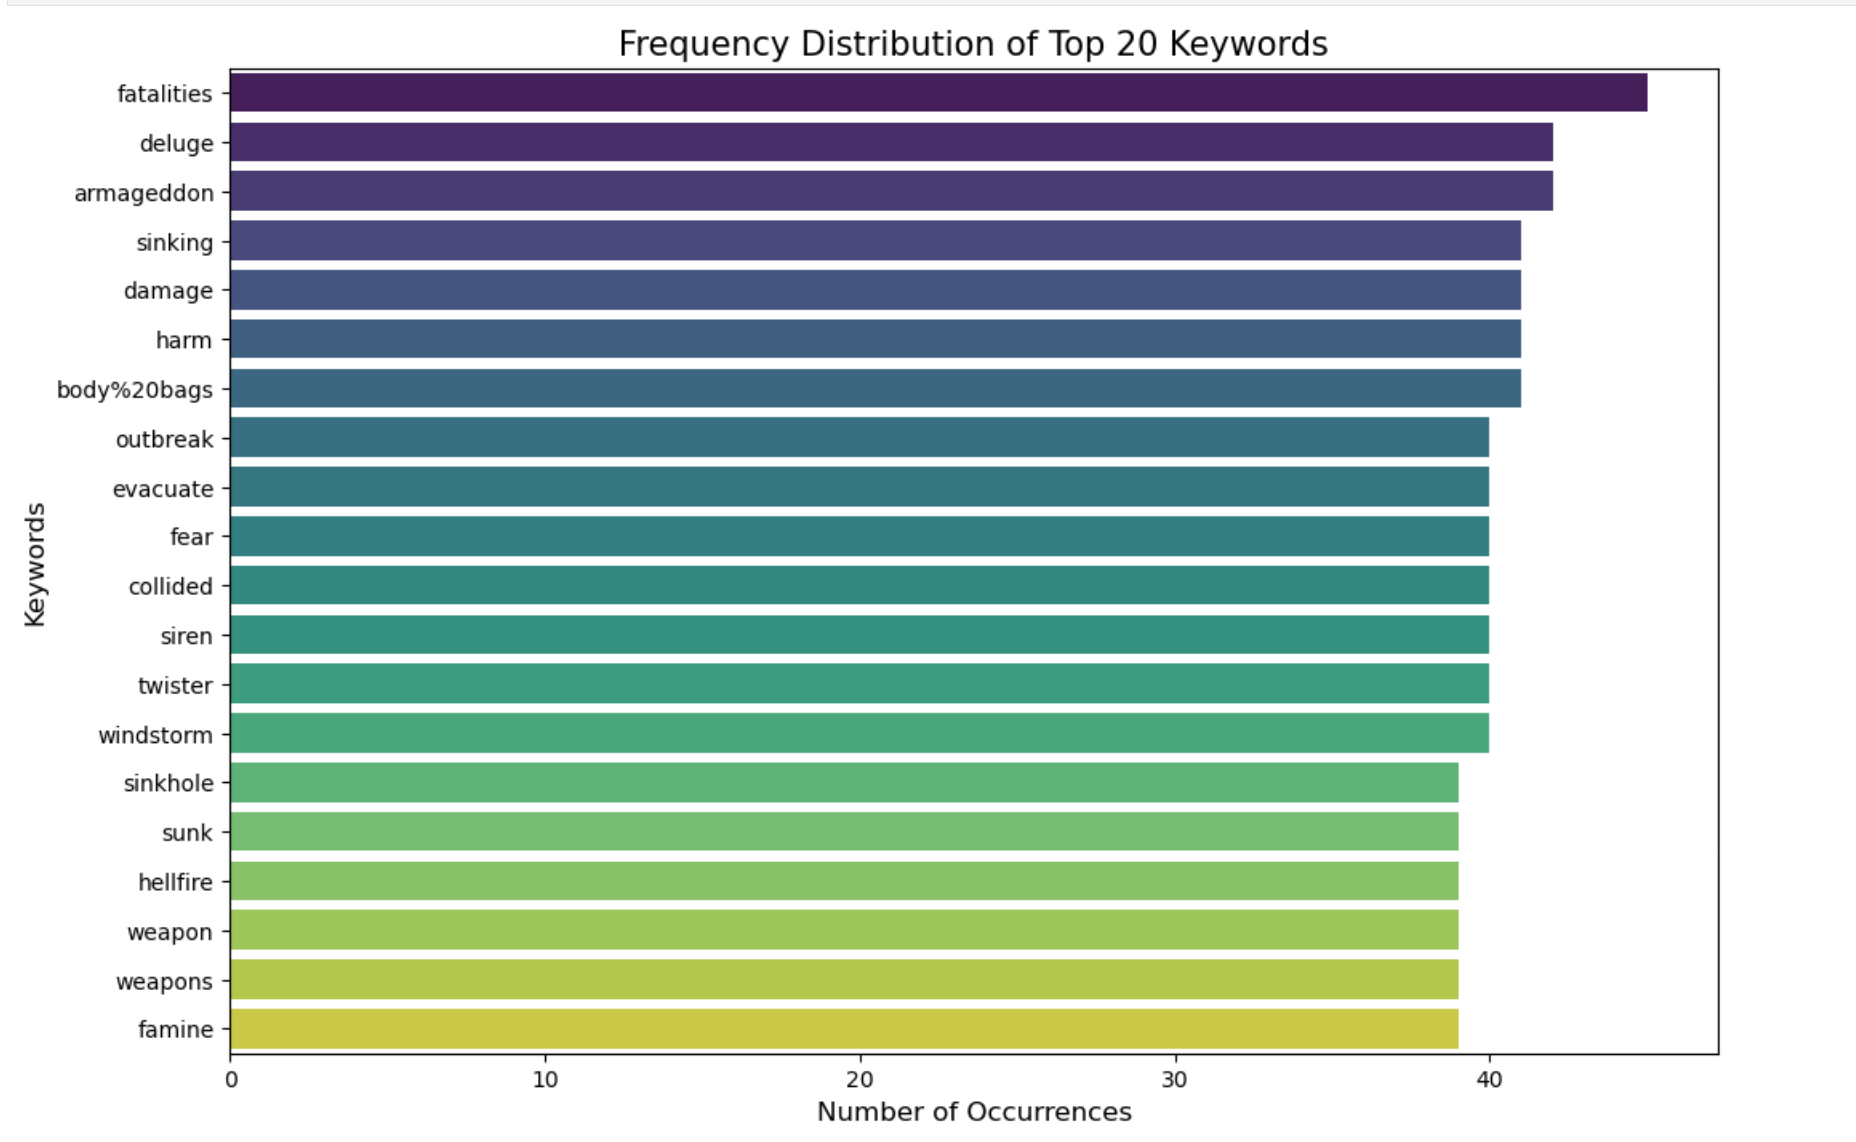
\includegraphics[width=0.8\textwidth]{top_20_disaster_keywords.png} 
    \caption{Top 20 Disaster Keywords}
    \label{fig:my_label}
\end{figure}
\paragraph{Furthermore, by looking at the frequency distribution, we can evaluate the kind of events that people are concerned about on the X platform.}
\section{Case Studies of Disaster Event Analysis using KDD}
\paragraph{In recent years, the ubiquity of social media platforms, particularly X, has transformed the landscape of disaster event analysis. With millions of users sharing real-time updates, tweets have become a valuable source of data for researchers and disaster response agencies alike.}
\paragraph{For example, recent papers \cite{nastaran_pourebrahim_ccfadf88} explored the role of X during Hurricane Sandy, focusing on the spatial-temporal distribution of tweets. By leveraging Natural Language Processing (NLP) techniques, they identified patterns related to the hurricane's path and impact areas, emphasizing the importance of geospatial analysis in disaster response. This study serves as a valuable benchmark for our analysis, as it underscores the potential of tweets as early warning indicators.}
\paragraph{Another groundbreaking study \cite{manuel_b__garcia_0996eb89} examined the sentiment of tweets during the COVID-19 epidemic. Through sentiment analysis, they discerned the evolution of public sentiment, from shock and panic during the early stages to hope and resilience in the aftermath. Such insights can guide public awareness campaigns, ensuring that messaging aligns with public sentiment during various disaster phases.}
\section{Conclusion: The Power of Tweets in Disaster Analysis}
\paragraph{Our journey through the KDD methodology with X's disaster tweets was both enlightening and impactful. We discovered that locations such as the USA, New York, and the United States emerged as significant hotspots for disaster-related discussions. Furthermore, themes revolving around fires, storms, emergencies, and fatalities provided insights into global disaster concerns.}
\paragraph{These findings underscore the potential of X as a real-time source of data, guiding disaster response strategies and public awareness campaigns. By understanding the pulse of the public through their tweets, stakeholders can make informed decisions, potentially mitigating the impact of future disaster events.}
\section{Future Directions in Disaster Event Analysis using KDD and Python}
\paragraph{The recent pioneering work in disaster sentiment analysis \cite{nastaran_pourebrahim_ccfadf88} and (Garcia, 2020) has paved the way for future research endeavors. By integrating geospatial analysis, as demonstrated in the Hurricane Sandy study, our project can delve deeper into the spatial-temporal distribution of tweets, potentially uncovering areas at immediate risk.}
\paragraph{Furthermore, sentiment analysis, as explored in the COVID-19 study, can offer a nuanced understanding of public sentiment during different disaster phases. Integrating such analysis can enable us to tailor public awareness campaigns, ensuring they resonate with the public's emotions and concerns.}
\paragraph{But beyond these technical advancements, our research holds the potential to drive societal change. By showcasing the power of tweets in disaster analysis, we can influence policymakers and disaster response agencies. Harnessing real-time data can revolutionize early warning systems, ensuring timely evacuations and resource deployments. Furthermore, our findings can inform public awareness campaigns, fostering a culture of preparedness and resilience.}
\paragraph{As researchers, we're not just uncovering patterns; we're laying the groundwork for a safer, more informed world. By collaborating with tech platforms, policymakers, and the public, we can harness the power of data to improve lives and shape a resilient future.}
\printbibliography
\end{document}